%\documentclass[11pt]{article}
\documentclass{article} % For LaTeX2e
\usepackage{nips12submit_e,times}

\usepackage{graphicx}
\usepackage{epsfig}
\usepackage{caption}
\usepackage{subcaption}
\usepackage{cite}
\usepackage{url}
\usepackage{wrapfig}

\newcommand{\fix}{\marginpar{FIX}}
\newcommand{\new}{\marginpar{NEW}}

\nipsfinaltrue

\begin{document}

\title{Clustering Learning on video sequences}

\author{
Eugenio Culurciello\thanks{More information on Eugenio Culurciello's laboratory and research can be found here: http://engineering.purdue.edu/elab/. Real time robotic vision systems: http://www.neuflow.org/} \\
Purdue University\\
\texttt{euge@purdue.edu} \\
\And
Jordan Bates \\
Purdue University\\
\texttt{jtbates@purdue.edu}
\AND
Jonghoon Jin \\
Purdue University\\
\texttt{jhjin@purdue.edu}
\AND
Aysegul Dundar \\
Purdue University\\
\texttt{adundar@purdue.edu}
\And
Clement Farabet \\
New York University \\
\texttt{cfarabet@nyu.edu}
}

%\date{\today}

\maketitle

\begin{abstract}
We present the clustering learning technique applied to video labeling with multi-layer feedforward deep neural networks. We show that networks trained with clustering learning on video segments can obtain similar levels of performance as supervised deep network trained to recognize faces in still frames. 
\end{abstract}


\section{Introduction}

Most scientists and engineers are fascinated by the design of an artificial vision system that can reproduce some of the human visual system capabilities in detecting, categorizing, tracking objects in view. The availability of a real-time synthetic vision system with such capabilities would find use in a large variety of applications, such as: autonomous cars, co-robots helpers, smart appliances, cellular-phones, to name a few.
 
In the recent years the fusion of bio-inspired and neuromorphic vision models with machine learning has dominated the development of artificial vision systems for the categorization of multiple objects in static frames.
Bio-inspired deep networks are computer-vision and computational-neuroscience models of the mammalian visual system implemented in deep neural networks \cite{lecun_gradient-based_1998,hadsell_dimensionality_2006,gregor_structured_2011,riesenhuber_hierarchical_1999,serre_feedforward_2007,serre_neuromorphic_2010}. Most deep network architectures are composed of multiple layers (2, 3 typically), where each layer is composed of: linear two-dimensional filtering, non-linearity, pooling of data, output data normalization \cite{jarrett_what_2009,lecun_convolutional_2010,boureau_theoretical_2010}. 
Recent machine learning research has focused on the task of training such deep networks from the abundant digital data available in the form of image frames and videos. In particular, deep networks need to learn good feature representations for complex visual tasks such as object categorization and tracking of objects in space and time, identifying object presence and absence. These representations usually involve learning the linear filter weight values from labeled and unlabeled input data. Since labeled data is costly and often ridden with human errors \cite{karpathy_lessons_2011, torralba_unbiased_2011, hou_meta-theory_2012}, the recent focus is on learning these features purely from unlabeled input data \cite{olshausen_emergence_1996, hyvarinen_independent_2000, hinton_fast_2006, vincent_extracting_2008, coates_analysis_2011}. These recent methods typically learn multiple layers of deep networks by training several layers of features, one layer at a time, with varying complexity of learning models. Traditional work in deep learning for vision has mostly focused on improving the learning algorithms, and rarely it has shown potential for overcoming some of the limitation of these systems, such as reliance on large sets of labeled data, and real-time operation for embedded systems.

Recent techniques based on unsupervised clustering algorithms are especially promising because they use simple learning methods that quickly converge \cite{coates_analysis_2011}. 
These algorithms are easy to setup and train and are especially suited for robotics research, because less complex knowledge of machine learning is needed, environment-specific data can be collected quickly with a few minutes of video, setup of custom size deep networks is quick and can be adapted to specific tasks. %reword this sentence?
In addition, real-time operation with efficient networks can be obtained with only a few minutes of training and setup, leading to quick and direct experimentation in robotic experiments.

In this paper we present unsupervised clustering algorithms applied to video sequences to perform training and operation of deep neural networks for general-purpose vision systems. 
The main goal of the paper is not to present state-of-art results on a specific dataset. Rather we want to present ways to quickly process video sequences to extract a large portion of information without the need of supervision and heavy learning techniques.
The goal is also to show that compact video-based unsupervised networks can support at least ten frames-per-second operation on commercial hardware, such as recent laptop computers.

The paper presents the following key innovations: (1) use of clustering learning for learning features from video with fully unsupervised techniques (Section \ref{}), (2) the ability of trained network to perform as well as supervised networks trained on still frames, (3) ability to run in real-time?. 



\section{Methods}
\label{sec-methods}

In this paper we created and tested a model of unsupervised clustering algorithms for video sequences (CL-video) that can quickly learn network parameters, and also is amenable to real-time operation with conventional mobile hardware.
We used the Torch7 software for all our experiments \cite{collobert_torch7_2011}, since this software can reduce training and learning of deep networks by 5-10 times compared to similar Matlab and Python tools.


\subsection{Input data}

We use input color video sequences of people talking in front of a camera as captured from a computer camera. The input video was resized to 120x 80 pixels and was contrast normalized separately on each RGB channel with a 9x9 gaussian filter using the Torch7 "nn.Spatial Contrastive Normalization" function.

We use the NYU face detector dataset to test how the unsupervised network would perform on labeled data. The NYU face dataset has a training size of 52,684 32x32 images and a test size of 5,854 32x32 images. The dataset has two classes: 'face' and 'background'. Input data was contrast normalized separately on each RGB channel with a 9x9 gaussian filter using the Torch7 "nn.Spatial Contrastive Normalization" function.

\begin{figure}
        \centering
        \begin{subfigure}[b]{0.5\textwidth}
                \centering
                
\includegraphics[width=2.65in]{fig-examplevideo.png}
                \caption{Example frame of the training video sequence.}
        \end{subfigure}%
        ~%add desired spacing between images, e. g. ~, \quad, \qquad etc. 
          %(or a blank line to force the subfigure onto a new line)
        \begin{subfigure}[b]{0.5\textwidth}
                \centering
                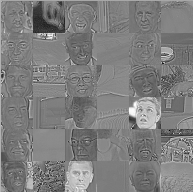
\includegraphics[width=2in]{fig-faceds.png}
                \caption{Examples from the NYU face dataset.}
        \end{subfigure}
        \caption{}
\end{figure}

Even if other groups showed slight improvements using the YUV color space \cite{jarrett_what_2009}, we did not use it. Rather, we kept the images in their original RGB to keep the model closer to biological human vision, where the retina is broadly sensitive to roughly RGB \cite{wandell_foundations_1995}. 

Also we did not use whitening of data (such as ZCA whitening) even if other groups have shown clear advantages of using it.  We did not use whitening because of two main reasons: first, it is not applicable for general-purpose vision system where an a-priori dataset cannot be obtained. Second, whitening computation is very expensive (similar to the first layer of a convolutional neural network) and we instead replaced it with local contrast normalization, which is a bio-inspired technique to whiten the input data removing its mean bias and adapting the input dynamic range.



\subsection{Network architecture}
\label{sec-net-arch}

We experimented by training an unsupervised deep neural network with 2 layers, not counting pooling and normalization operations. The two layers were composed of a two-dimensional convolutional linear filtering stage, a spatial max pooling stage, and a subtractive and/or divisive normalization layer for removing the mean and resetting the std of all outputs to unity. 
The filters of the first two layers are generated with unsupervised clustering algorithms, as explained below. 
Using the naming convention in \cite{lecun_convolutional_2010}, for each layer $l$  $x_i$ is an input feature map, $y_i$ is an output feature map. The input of each layer is a 3D array with $n_l$ 2D feature maps of size $n_{l1} \cdot n_{l2}$. Each component (pixel, neuron) is denoted $x_{ijk}$. The output is also a 3D array, $y_i$ composed of $m_l$ feature maps of size $m_{l1} \cdot m_{l2}$.

The layers in the clustering learning network used the following sequence of operations:
\begin{enumerate}
\item Volumetric Convolution module (1st layer): performing convolutions on images with the learned volumetric CL filters
\item Spatial Convolution module (2nd layer): performing convolutions on images with the learned CL filters: $yc_i=b_j+\sum_i{k_{ij}\ast x_i}$, where $\ast$ is the 2D discrete convolution operator and $b_j$ is a trainable bias parameter.
\item Spatial Max Pooling module: $yp_i = max_{n \times n}(yc_{ij})$ with $n =  2$ in this work.
\item Hyperbolic tangent nonlinearity: $ynl_i = tanh(yp_i )$
\item Spatial Subtractive or Contrastive Normalization: to zero the data mean, reset std to unity. The subtractive normalization operation for a given site $ynl_{ijk}$ computes: $v_{ijk} = ynl_{ijk} - \sum_{ipq} w_{pq} \cdot ynl_{i,j+p,k+q}$, where $w_{pq}$ is a normalized truncated Gaussian weighting window (typically of size 9x9). The divisive normalization computes $y_{ijk} = v_{ijk}/max(mean(\sigma_{jk}),\sigma_{jk})$ where $\sigma_{jk} = (\sum_{ipq} w_{pq} \cdot v^2_{i,j+p,k+q})^{1/2}$. The local contrast normalization layer is inspired by visual neuroscience models.
\end{enumerate}


All networks used 32 filters on the first layer, 64 filters on the second layer. Clustering learning networks used a fully connected input to 1st, and 1st to 2nd layer. We experimented with SLAC connections \cite{coates2012emergence}. In this case we used 4x more features than the numbers given above as beginning features, and then we decreased them to the same size of 32,64 in each respective layer. After the Convolution modules we added a SpatialMaxMap module to compute the groups and reduce the feature numbers.



\subsection{Learning}
We use k-means clustering algorithm (we refer to this step as \textit{Clustering Learning algorithm}) to learn a set of 32 filters in the first layer, and 64 filters in the second layer. The techniques and scripts are general and can quickly modified to learn any number of filters. The filter sizes on both layers was set to 5 x 5 pixels.
The input video was sampled to obtain 10,000 patches at random locations of size 5 x 5. These patches were used by the Clustering Learning algorithm to train the first layer, using 15 epochs on the patches dataset and 1,000 mini batch updates for the k-means algorithm. We learned Volumetric filters by sampling the same image location on contiguous $N_f$ frames. Then we grouped the 5 x 5 x $N_f$ frames in one vector and passed it to the Clustering Learning module to perform k-means clustering. This provided volumetric filters that were then unpacked into 5 x 5 patches for each of the input $N_f$ frames. $N_f$ frames were then input into the VolumetricConvolution module to provide 32 output spatio-temporal feature maps. These are also commonly referred as "motion filters" because they can be used as optical-flow detectors on video sequences.

The input video dataset was processed first by the 1st Volumetric layer, then the output was again sampled by taking 100,000 patches at random locations one random of the 32 feature maps. We then applied the Clustering Learning algorithm again to obtain the required 64 filters for the second layer. These filter were no Volumetric, but were computed on single maps. 

\begin{figure}
\centering
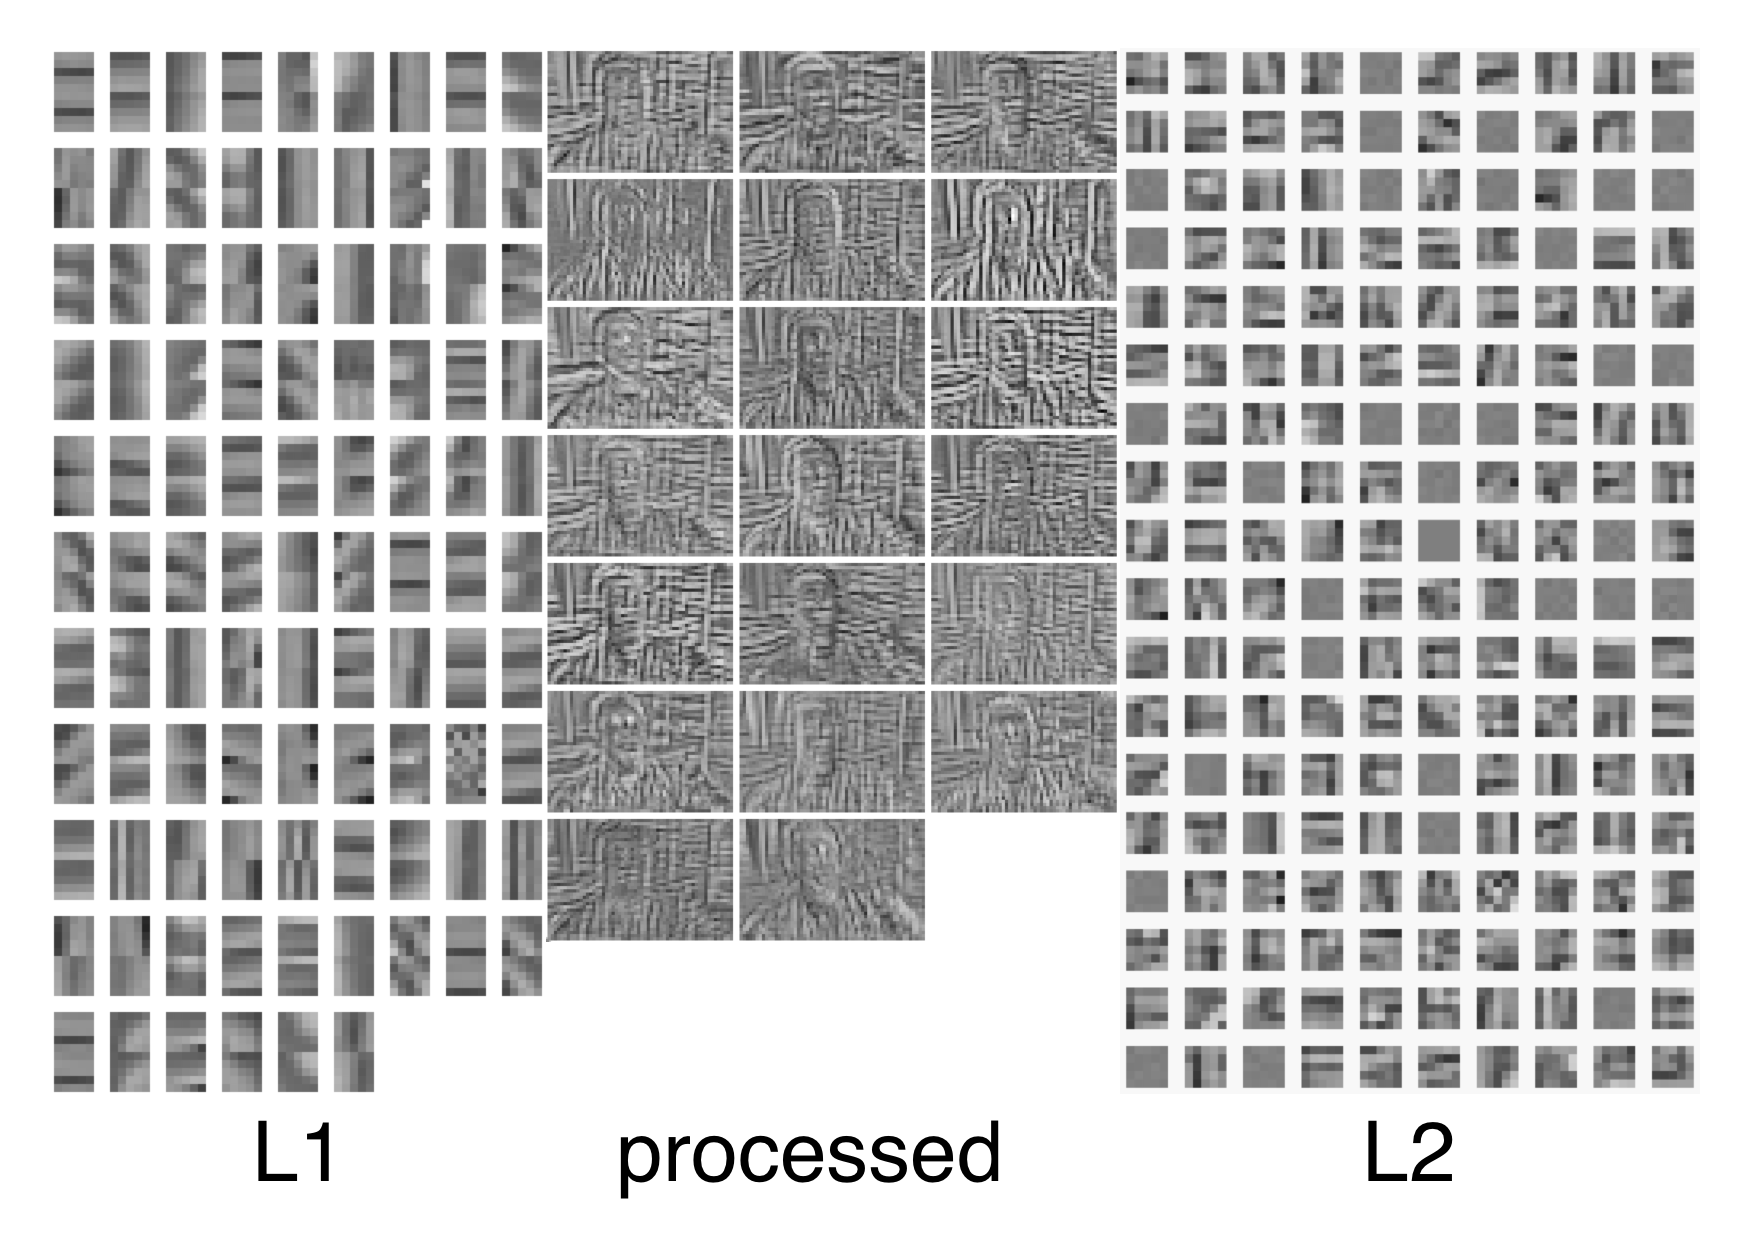
\includegraphics[width=5in]{fig-filtersproc.png}
\caption{Layer 1 filters; processed frames with layer 1 filters; layer 2 filters.}
\label{fig-filterproc}
\end{figure}


Examples of the filters learned with the CL technique on a 1st and 2nd layer are given in figure \ref{fig-filterproc}. The volumetric filters are shown on the left of the figure as 5 x 5 x 2 columns, since we used 2 frames in this example figure. We can provide animated-GIF files upon request. We also show in in figure \ref{fig-filterproc}-middle samples of the processed  1st layer outputs. We also report on the right of the figure the 2nd layer filters. These 2nd layer filters are just a subset of the 32 x 64 filter learned with Clustering Learning. We learned this many filters because layer 1 and 2 are fully connected, and thus can benefit from this large number of different filters. This is different from the approach taken by \ref{coates2012learning,coates2012learning} where the output of the 1st layer was reshaped to a vector and fed to the k-means algorithm, thus doing away with inter-network connection matrices. 

Both layer filters were obtained with training for ~10 minutes on a modern quad-core Intel i7 laptop. A supervised network of this size would require several tens of thousands of image examples and several hours of training time.

\begin{wrapfigure}{r}{.2\textwidth}
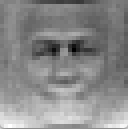
\includegraphics[width=1.2in]{fig-bestnface.png}
\caption{Top neuron encoding for a face found after training the CL-video 2-layer network unsupervised.}
\label{fig-bestnface}
\end{wrapfigure}

In order to test the network after training, we then used the unsupervised deep network to process a dataset of face from NYU. We passed both the test and train sets through the network. The ~30,000 32 x 32 images were processed in about 7 minutes on a modern quad-core Intel i7 laptop running Torch7. We the used a linear layer (linear regression) and trained it on the 64 x 2 x 2 outputs of the processed face dataset. We used the train set for training. We then verified the precision of the network on the test set.
As input to the Volumetric networks, we gave the same input to all required frames, but copying the same input samples $N_f$ times. This is not the best test for a Volumetric network that learned spatio-temporal filters, and we are working on more tests with video datasets.

In order to test the ability of our network to learn frequently occurring objects in the video scene, we tested the output of the network after processing the entire NYU face dataset with it. We then found the neuron that in overall responded the most to a face, but not a background. We found the neuron most responsive to face $tn$ by running obtaining the maximum of all output neuron of the network $net$ to the face set, as can be seen in the equation below. 

\begin{equation}
bf = \sum_i tn(i) \cdot dataset(i),  tn = arg_n max( \sum_i net_n(faceset(i) ) )
\end{equation}

We then computed a weighted average of $tn$ with the output of the network for each sample of the dateaset, be that a face or a background. The weighted average neuron $bf$ also reported in the equation above. The optimal stimulus for the neuron $bf$ is reported in figure \ref{fig-bestnface}.


%Larger network:
%This network can be executed in real-time with accelerated hardware [neuflow]



\section{Results}
\label{sec-results}


We report the results of our experiments in table \ref{table1}. We here compared several version of the unsupervised 2-layer deep network. 

\begin{table}[htdp]
\caption{Results.}
\begin{center}
\begin{tabular}{|c|c|c|c|c|c|c|}
\hline\hline
1L filters	& 2L filters	& type	& Frames	& Precision Tot. & Precision Face  & Precision Bg. \\ 
\hline
32 		& 64 		& full					& 1	& 94.92  		& 92.26		& 97.58  \\
32 		& 64 		& full LCN				& 1	& 97.07 		& 97.89		& 99.13  \\
64		& 128	& full LCN				& 1	& 98.41		& 97.23		& 99.59 \\
32 		& 64 		& full	 LCN				& 2	& 95.74		& 95.11		& 98.83  \\
32 		& 64 		& full LCN				& 4	& 93.16  		& 95.78		& 97.13  \\ 
32 		& 64 		& full LCN noVC	& 2	& \bf{97.95}  	& 97.24		& 98.67  \\ 
128 $\rightarrow$ 32 	& 64 		& SLAC 1L			& 1	& 95.21  		& 92.60		& 97.81  \\
128 $\rightarrow$ 32 	& 64 		& SLAC 1L, LCN		& 1	& 97.63 		& 98.17		& 99.43  \\ 
128 $\rightarrow$ 32 	& 256 $\rightarrow$ 64 	& SLAC 2L		& 1	& 93.16 		& 91.20		& 95.11  \\ 
32 		& 64 		& random				& 1	& 93.16 		& 91.20		& 95.11  \\ 
8 		& 32 		& supervised CNN		& 1	& 99.35 		& 99.16		& 99.53  \\ 
32x32 	& -- 		& linear on pixels		& 1	& 79.30 		& 83.71		& 93.24  \\ 
\hline\hline
\end{tabular}
\end{center}
\label{table1}
\end{table}


The size of the network, the number of each layer of filters,  is given in the table. The type of network was: full = fully connected; LCN = local contrast normalization at the output of each layer (as opposed to a simpler subtractive normalization of the means only); SLAC = single-link agglomerate clustering technique from \cite{coates2012learning} to reduce the filters from 128 to 32 on the 1st layer and from 256 to 64 in the 2nd layer; random = test of a random network to compare the learning techniques; noVC does not compute volumetric filters, but rather uses the same static filters at each frame ;supervised CNN = standard 2-layer convolutional neural network used as face detector with 8 features on the 1st layer and 32 on the second layer, max pooling of 4 x 4, connection table with fan in of 8, followed by a linear classifier; linear on pixels = test of a linear classifier on the bare 32 x 32 input pixels without the use of any deep network for feature extraction.

With only one frame as input SLAC 1-layer with LCN provided the best results, followed closely by the fully connected LCN network. It is clear that proper normalization of the standard deviation at each layer is key to the highest performance. This is due to the fact that this step prepares the best data spread for the nonlinearity at each layer, thus preserving the maximum information content. 

Similar results are reported by \cite{coates2012emergence}. 
The SLAC algorithm also performed well only on the 1st layer, and reported a loss of 2\% points when used in the second layer. This issue is not well understood and under investigation. 

Random networks gave surprisingly high results, as has been reported by several other groups \cite{saxe2011random}. But the Clustering Learning algorithm was in overall superior.  The random network architecture was identical to a 32, 64 full LCN model, with weights initialized with a random uniform distribution by the Torch7 package.

A linear layer on the input image was computed as a baseline to give indication of the difficulty of the task. As expected, a face-detection task is hardly the best example for a deep network with much larger capacity. nevertheless the ease of availability of data and the fact that our network was able to learn face features from video is a satisfactory result. In any case the linear network performed much worse at 79\% recognition rate on faces. almost 20 points lower than Clustering Learning networks.

The supervised CNN gave the top results with above 99\% recognition rates, and by using a smaller network. This is also expected, as gradient descent algorithms are the best at adapting a network architecture to a single task. But we remind the reader that our goal is a general network with little need for supervision, so we are willing to accept a less efficient network for these great advantages. 

The best results of this study was achieved with a fully-connected network with LCN and without the use of Volumetric filters. This network instead computed static filters and used them at each frame. This idea overcomes the problems of feeding a video as input and training on a static dataset, and allows to show the full power of Clustering Learning applied to videos: the ability to cluster features even across frames, be those frames from video or still images.

Notice also that in the case of the fully connected network, we also trained and tested a Volumetric network with 1,2,4 input frames. 
2 frames showed increased recognition results, due to the fast that the two frames give higher signal-to-noise ratio at the input of the network. 4 frames instead did not perform as well. Partly this is due to the fact that our test dataset was not a video, so most of the learnt spatio-temporal filters were not effectively used in testing.

\begin{table}[htdp]
\caption{Network execution time on a 320 x 240 frame.}
\begin{center}
\begin{tabular}{|c|c|c|c|c|}
\hline\hline
1L filters	& 2L filters	& type				& frames 		&time [ms] \\ 
\hline
32 		& 64 			& full					& 1			& 356.50 \\
32 		& 64 			& full LCN				& 1			& 421.37 \\
32 		& 64 			& full	 LCN				& 2			& 560.45 \\
32 		& 64 			& full	 LCN				& 4			& 858.28 \\
128 $\rightarrow$ 32 	& 64 			& SLAC 1L			& 1			& 654.25 \\
128 $\rightarrow$ 32 	& 256 $\rightarrow$ 64 	& SLAC 2L			& 1			& 1067 \\	
64		& 128		& full					& 1			& 1036 \\
8		& 32			& CNN				& 1			& 6.04 \\

\hline\hline
\end{tabular}
\end{center}
\label{table2}
\end{table}

Table \ref{table2} reports the execution time of some of the tested networks reported in table \ref{table1}.

Increasing the size of the filters to 64 and 128 also gave really high results, but with a slower computation time of about 1s.

The supervised CNN has the lowest computational time, together with the highest performance, as it is fully numerically optimized to the task and dataset by gradient descent methods, which currently perform the best on fixed dataset. If only fixed dataset performance would translate to real-life performance, there would not be a need for unsupervised training. But unfortunately this is not the case and  supervised CNN perform quite badly when used in a different setting from which they were trained for \cite{ec_cl_paper1}. We thus advocate to take the performance of  supervised CNN with a grain of salt: remember that its very high performance, at least its precision, will not be available as part of a general-purpose vision system.



\section{Discussion}

We presented results on clustering learning algorithms trained on video sequences for general-purpose vision system. These algorithms can be used to train multi-layer feed-forward neural networks from videos in minutes. We show results on 



%\section{TODO}
%


\subsubsection*{Acknowledgments}
We are especially grateful to the the Torch7 developing team, in particular Ronan Collobert, who first developed this great, easy and efficient tool, Clement Farabet, Koray Kavukcuoglu, Leon Bottou. We could not have done any of this work without standing on these giants shoulders.

\bibliography{clustering}
\bibliographystyle{unsrt}



\end{document}
